
%% bare_jrnl.tex
%% V1.4
%% 2012/12/27
%% by Michael Shell
%% see http://www.michaelshell.org/
%% for current contact information.
%%
%% This is a skeleton file demonstrating the use of IEEEtran.cls
%% (requires IEEEtran.cls version 1.8 or later) with an IEEE journal paper.
%%
%% Support sites:
%% http://www.michaelshell.org/tex/ieeetran/
%% http://www.ctan.org/tex-archive/macros/latex/contrib/IEEEtran/
%% and
%% http://www.ieee.org/



% *** Authors should verify (and, if needed, correct) their LaTeX system  ***
% *** with the testflow diagnostic prior to trusting their LaTeX platform ***
% *** with production work. IEEE's font choices can trigger bugs that do  ***
% *** not appear when using other class files.                            ***
% The testflow support page is at:
% http://www.michaelshell.org/tex/testflow/


%%*************************************************************************
%% Legal Notice:
%% This code is offered as-is without any warranty either expressed or
%% implied; without even the implied warranty of MERCHANTABILITY or
%% FITNESS FOR A PARTICULAR PURPOSE! 
%% User assumes all risk.
%% In no event shall IEEE or any contributor to this code be liable for
%% any damages or losses, including, but not limited to, incidental,
%% consequential, or any other damages, resulting from the use or misuse
%% of any information contained here.
%%
%% All comments are the opinions of their respective authors and are not
%% necessarily endorsed by the IEEE.
%%
%% This work is distributed under the LaTeX Project Public License (LPPL)
%% ( http://www.latex-project.org/ ) version 1.3, and may be freely used,
%% distributed and modified. A copy of the LPPL, version 1.3, is included
%% in the base LaTeX documentation of all distributions of LaTeX released
%% 2003/12/01 or later.
%% Retain all contribution notices and credits.
%% ** Modified files should be clearly indicated as such, including  **
%% ** renaming them and changing author support contact information. **
%%
%% File list of work: IEEEtran.cls, IEEEtran_HOWTO.pdf, bare_adv.tex,
%%                    bare_conf.tex, bare_jrnl.tex, bare_jrnl_compsoc.tex,
%%                    bare_jrnl_transmag.tex
%%*************************************************************************

% Note that the a4paper option is mainly intended so that authors in
% countries using A4 can easily print to A4 and see how their papers will
% look in print - the typesetting of the document will not typically be
% affected with changes in paper size (but the bottom and side margins will).
% Use the testflow package mentioned above to verify correct handling of
% both paper sizes by the user's LaTeX system.
%
% Also note that the "draftcls" or "draftclsnofoot", not "draft", option
% should be used if it is desired that the figures are to be displayed in
% draft mode.
%
\documentclass[journal]{IEEEtran}
%
% If IEEEtran.cls has not been installed into the LaTeX system files,
% manually specify the path to it like:
% \documentclass[journal]{../sty/IEEEtran}





% Some very useful LaTeX packages include:
% (uncomment the ones you want to load)


% *** MISC UTILITY PACKAGES ***
%
%\usepackage{ifpdf}
% Heiko Oberdiek's ifpdf.sty is very useful if you need conditional
% compilation based on whether the output is pdf or dvi.
% usage:
% \ifpdf
%   % pdf code
% \else
%   % dvi code
% \fi
% The latest version of ifpdf.sty can be obtained from:
% http://www.ctan.org/tex-archive/macros/latex/contrib/oberdiek/
% Also, note that IEEEtran.cls V1.7 and later provides a builtin
% \ifCLASSINFOpdf conditional that works the same way.
% When switching from latex to pdflatex and vice-versa, the compiler may
% have to be run twice to clear warning/error messages.






% *** CITATION PACKAGES ***
%
%\usepackage{cite}
% cite.sty was written by Donald Arseneau
% V1.6 and later of IEEEtran pre-defines the format of the cite.sty package
% \cite{} output to follow that of IEEE. Loading the cite package will
% result in citation numbers being automatically sorted and properly
% "compressed/ranged". e.g., [1], [9], [2], [7], [5], [6] without using
% cite.sty will become [1], [2], [5]--[7], [9] using cite.sty. cite.sty's
% \cite will automatically add leading space, if needed. Use cite.sty's
% noadjust option (cite.sty V3.8 and later) if you want to turn this off
% such as if a citation ever needs to be enclosed in parenthesis.
% cite.sty is already installed on most LaTeX systems. Be sure and use
% version 4.0 (2003-05-27) and later if using hyperref.sty. cite.sty does
% not currently provide for hyperlinked citations.
% The latest version can be obtained at:
% http://www.ctan.org/tex-archive/macros/latex/contrib/cite/
% The documentation is contained in the cite.sty file itself.






% *** GRAPHICS RELATED PACKAGES ***
%
\ifCLASSINFOpdf
  % \usepackage[pdftex]{graphicx}
  % declare the path(s) where your graphic files are
  % \graphicspath{{../pdf/}{../jpeg/}}
  % and their extensions so you won't have to specify these with
  % every instance of \includegraphics
  % \DeclareGraphicsExtensions{.pdf,.jpeg,.png}
\else
  % or other class option (dvipsone, dvipdf, if not using dvips). graphicx
  % will default to the driver specified in the system graphics.cfg if no
  % driver is specified.
  % \usepackage[dvips]{graphicx}
  % declare the path(s) where your graphic files are
  % \graphicspath{{../eps/}}
  % and their extensions so you won't have to specify these with
  % every instance of \includegraphics
  % \DeclareGraphicsExtensions{.eps}
\fi
% graphicx was written by David Carlisle and Sebastian Rahtz. It is
% required if you want graphics, photos, etc. graphicx.sty is already
% installed on most LaTeX systems. The latest version and documentation
% can be obtained at: 
% http://www.ctan.org/tex-archive/macros/latex/required/graphics/
% Another good source of documentation is "Using Imported Graphics in
% LaTeX2e" by Keith Reckdahl which can be found at:
% http://www.ctan.org/tex-archive/info/epslatex/
%
% latex, and pdflatex in dvi mode, support graphics in encapsulated
% postscript (.eps) format. pdflatex in pdf mode supports graphics
% in .pdf, .jpeg, .png and .mps (metapost) formats. Users should ensure
% that all non-photo figures use a vector format (.eps, .pdf, .mps) and
% not a bitmapped formats (.jpeg, .png). IEEE frowns on bitmapped formats
% which can result in "jaggedy"/blurry rendering of lines and letters as
% well as large increases in file sizes.
%
% You can find documentation about the pdfTeX application at:
% http://www.tug.org/applications/pdftex





% *** MATH PACKAGES ***
%
%\usepackage[cmex10]{amsmath}
% A popular package from the American Mathematical Society that provides
% many useful and powerful commands for dealing with mathematics. If using
% it, be sure to load this package with the cmex10 option to ensure that
% only type 1 fonts will utilized at all point sizes. Without this option,
% it is possible that some math symbols, particularly those within
% footnotes, will be rendered in bitmap form which will result in a
% document that can not be IEEE Xplore compliant!
%
% Also, note that the amsmath package sets \interdisplaylinepenalty to 10000
% thus preventing page breaks from occurring within multiline equations. Use:
%\interdisplaylinepenalty=2500
% after loading amsmath to restore such page breaks as IEEEtran.cls normally
% does. amsmath.sty is already installed on most LaTeX systems. The latest
% version and documentation can be obtained at:
% http://www.ctan.org/tex-archive/macros/latex/required/amslatex/math/





% *** SPECIALIZED LIST PACKAGES ***
%
%\usepackage{algorithmic}
% algorithmic.sty was written by Peter Williams and Rogerio Brito.
% This package provides an algorithmic environment fo describing algorithms.
% You can use the algorithmic environment in-text or within a figure
% environment to provide for a floating algorithm. Do NOT use the algorithm
% floating environment provided by algorithm.sty (by the same authors) or
% algorithm2e.sty (by Christophe Fiorio) as IEEE does not use dedicated
% algorithm float types and packages that provide these will not provide
% correct IEEE style captions. The latest version and documentation of
% algorithmic.sty can be obtained at:
% http://www.ctan.org/tex-archive/macros/latex/contrib/algorithms/
% There is also a support site at:
% http://algorithms.berlios.de/index.html
% Also of interest may be the (relatively newer and more customizable)
% algorithmicx.sty package by Szasz Janos:
% http://www.ctan.org/tex-archive/macros/latex/contrib/algorithmicx/




% *** ALIGNMENT PACKAGES ***
%
%\usepackage{array}
% Frank Mittelbach's and David Carlisle's array.sty patches and improves
% the standard LaTeX2e array and tabular environments to provide better
% appearance and additional user controls. As the default LaTeX2e table
% generation code is lacking to the point of almost being broken with
% respect to the quality of the end results, all users are strongly
% advised to use an enhanced (at the very least that provided by array.sty)
% set of table tools. array.sty is already installed on most systems. The
% latest version and documentation can be obtained at:
% http://www.ctan.org/tex-archive/macros/latex/required/tools/


% IEEEtran contains the IEEEeqnarray family of commands that can be used to
% generate multiline equations as well as matrices, tables, etc., of high
% quality.




% *** SUBFIGURE PACKAGES ***
%\ifCLASSOPTIONcompsoc
%  \usepackage[caption=false,font=normalsize,labelfont=sf,textfont=sf]{subfig}
%\else
%  \usepackage[caption=false,font=footnotesize]{subfig}
%\fi
% subfig.sty, written by Steven Douglas Cochran, is the modern replacement
% for subfigure.sty, the latter of which is no longer maintained and is
% incompatible with some LaTeX packages including fixltx2e. However,
% subfig.sty requires and automatically loads Axel Sommerfeldt's caption.sty
% which will override IEEEtran.cls' handling of captions and this will result
% in non-IEEE style figure/table captions. To prevent this problem, be sure
% and invoke subfig.sty's "caption=false" package option (available since
% subfig.sty version 1.3, 2005/06/28) as this is will preserve IEEEtran.cls
% handling of captions.
% Note that the Computer Society format requires a larger sans serif font
% than the serif footnote size font used in traditional IEEE formatting
% and thus the need to invoke different subfig.sty package options depending
% on whether compsoc mode has been enabled.
%
% The latest version and documentation of subfig.sty can be obtained at:
% http://www.ctan.org/tex-archive/macros/latex/contrib/subfig/




% *** FLOAT PACKAGES ***
%
%\usepackage{fixltx2e}
% fixltx2e, the successor to the earlier fix2col.sty, was written by
% Frank Mittelbach and David Carlisle. This package corrects a few problems
% in the LaTeX2e kernel, the most notable of which is that in current
% LaTeX2e releases, the ordering of single and double column floats is not
% guaranteed to be preserved. Thus, an unpatched LaTeX2e can allow a
% single column figure to be placed prior to an earlier double column
% figure. The latest version and documentation can be found at:
% http://www.ctan.org/tex-archive/macros/latex/base/


%\usepackage{stfloats}
% stfloats.sty was written by Sigitas Tolusis. This package gives LaTeX2e
% the ability to do double column floats at the bottom of the page as well
% as the top. (e.g., "\begin{figure*}[!b]" is not normally possible in
% LaTeX2e). It also provides a command:
%\fnbelowfloat
% to enable the placement of footnotes below bottom floats (the standard
% LaTeX2e kernel puts them above bottom floats). This is an invasive package
% which rewrites many portions of the LaTeX2e float routines. It may not work
% with other packages that modify the LaTeX2e float routines. The latest
% version and documentation can be obtained at:
% http://www.ctan.org/tex-archive/macros/latex/contrib/sttools/
% Do not use the stfloats baselinefloat ability as IEEE does not allow
% \baselineskip to stretch. Authors submitting work to the IEEE should note
% that IEEE rarely uses double column equations and that authors should try
% to avoid such use. Do not be tempted to use the cuted.sty or midfloat.sty
% packages (also by Sigitas Tolusis) as IEEE does not format its papers in
% such ways.
% Do not attempt to use stfloats with fixltx2e as they are incompatible.
% Instead, use Morten Hogholm'a dblfloatfix which combines the features
% of both fixltx2e and stfloats:
%
% \usepackage{dblfloatfix}
% The latest version can be found at:
% http://www.ctan.org/tex-archive/macros/latex/contrib/dblfloatfix/




%\ifCLASSOPTIONcaptionsoff
%  \usepackage[nomarkers]{endfloat}
% \let\MYoriglatexcaption\caption
% \renewcommand{\caption}[2][\relax]{\MYoriglatexcaption[#2]{#2}}
%\fi
% endfloat.sty was written by James Darrell McCauley, Jeff Goldberg and 
% Axel Sommerfeldt. This package may be useful when used in conjunction with 
% IEEEtran.cls'  captionsoff option. Some IEEE journals/societies require that
% submissions have lists of figures/tables at the end of the paper and that
% figures/tables without any captions are placed on a page by themselves at
% the end of the document. If needed, the draftcls IEEEtran class option or
% \CLASSINPUTbaselinestretch interface can be used to increase the line
% spacing as well. Be sure and use the nomarkers option of endfloat to
% prevent endfloat from "marking" where the figures would have been placed
% in the text. The two hack lines of code above are a slight modification of
% that suggested by in the endfloat docs (section 8.4.1) to ensure that
% the full captions always appear in the list of figures/tables - even if
% the user used the short optional argument of \caption[]{}.
% IEEE papers do not typically make use of \caption[]'s optional argument,
% so this should not be an issue. A similar trick can be used to disable
% captions of packages such as subfig.sty that lack options to turn off
% the subcaptions:
% For subfig.sty:
% \let\MYorigsubfloat\subfloat
% \renewcommand{\subfloat}[2][\relax]{\MYorigsubfloat[]{#2}}
% However, the above trick will not work if both optional arguments of
% the \subfloat command are used. Furthermore, there needs to be a
% description of each subfigure *somewhere* and endfloat does not add
% subfigure captions to its list of figures. Thus, the best approach is to
% avoid the use of subfigure captions (many IEEE journals avoid them anyway)
% and instead reference/explain all the subfigures within the main caption.
% The latest version of endfloat.sty and its documentation can obtained at:
% http://www.ctan.org/tex-archive/macros/latex/contrib/endfloat/
%
% The IEEEtran \ifCLASSOPTIONcaptionsoff conditional can also be used
% later in the document, say, to conditionally put the References on a 
% page by themselves.




% *** PDF, URL AND HYPERLINK PACKAGES ***
%
%\usepackage{url}
% url.sty was written by Donald Arseneau. It provides better support for
% handling and breaking URLs. url.sty is already installed on most LaTeX
% systems. The latest version and documentation can be obtained at:
% http://www.ctan.org/tex-archive/macros/latex/contrib/url/
% Basically, \url{my_url_here}.




% *** Do not adjust lengths that control margins, column widths, etc. ***
% *** Do not use packages that alter fonts (such as pslatex).         ***
% There should be no need to do such things with IEEEtran.cls V1.6 and later.
% (Unless specifically asked to do so by the journal or conference you plan
% to submit to, of course. )


% correct bad hyphenation here
\hyphenation{op-tical net-works semi-conduc-tor}

% Add the listings package for code formatting
\usepackage{listings}

\usepackage{graphicx} % Required for the inclusion of images



\begin{document}
%
% paper title
% can use linebreaks \\ within to get better formatting as desired
% Do not put math or special symbols in the title.
\title{Project Report for Cpr E 583}
%
%
% author names and IEEE memberships
% note positions of commas and nonbreaking spaces ( ~ ) LaTeX will not break
% a structure at a ~ so this keeps an author's name from being broken across
% two lines.
% use \thanks{} to gain access to the first footnote area
% a separate \thanks must be used for each paragraph as LaTeX2e's \thanks
% was not built to handle multiple paragraphs
%

\author{Blake~Vermeer,
        Piriya~Kris~Hall,
        and~Rohit~Zambre}% <-this % stops a space
%\thanks{M. Shell is with the Department
%of Electrical and Computer Engineering, Georgia Institute of Technology, Atlanta,
%GA, 30332 USA e-mail: (see http://www.michaelshell.org/contact.html).}% <-this % stops a space
%\thanks{J. Doe and J. Doe are with Anonymous University.}% <-this % stops a space
%\thanks{Manuscript received April 19, 2005; revised December 27, 2012.}}

% note the % following the last \IEEEmembership and also \thanks - 
% these prevent an unwanted space from occurring between the last author name
% and the end of the author line. i.e., if you had this:
% 
% \author{....lastname \thanks{...} \thanks{...} }
%                     ^------------^------------^----Do not want these spaces!
%
% a space would be appended to the last name and could cause every name on that
% line to be shifted left slightly. This is one of those "LaTeX things". For
% instance, "\textbf{A} \textbf{B}" will typeset as "A B" not "AB". To get
% "AB" then you have to do: "\textbf{A}\textbf{B}"
% \thanks is no different in this regard, so shield the last } of each \thanks
% that ends a line with a % and do not let a space in before the next \thanks.
% Spaces after \IEEEmembership other than the last one are OK (and needed) as
% you are supposed to have spaces between the names. For what it is worth,
% this is a minor point as most people would not even notice if the said evil
% space somehow managed to creep in.



% The paper headers
\markboth{CprE 583 Project Report}%
{CprE 583 Project Report}
% The only time the second header will appear is for the odd numbered pages
% after the title page when using the twoside option.
% 
% *** Note that you probably will NOT want to include the author's ***
% *** name in the headers of peer review papers.                   ***
% You can use \ifCLASSOPTIONpeerreview for conditional compilation here if
% you desire.




% If you want to put a publisher's ID mark on the page you can do it like
% this:
%\IEEEpubid{0000--0000/00\$00.00~\copyright~2012 IEEE}
% Remember, if you use this you must call \IEEEpubidadjcol in the second
% column for its text to clear the IEEEpubid mark.



% use for special paper notices
%\IEEEspecialpapernotice{(Invited Paper)}




% make the title area
\maketitle

% As a general rule, do not put math, special symbols or citations
% in the abstract or keywords.
\begin{abstract}
This paper outlines the attempt at creating a hardware accelerator for the generation of a chain of large prime numbers, known as a Cunningham chain. The motivation for this project came from a cryptocurrency called Primecoin, specifically its proof-of-work. Primecoin accepts as a proof-of-work a Cunningham chain of the first or second kind, as well as a Bi-twin chain. To this date there have been little public success with hardware acceleration of the mining of this cryptocurrency. This project was an attempt to accelerate the generation and validation of Cunningham chains to be used with Primecoin. \\

\end{abstract}

% Note that keywords are not normally used for peerreview papers.
\begin{IEEEkeywords}
FPGA, primality test, Cunningham chain.
\end{IEEEkeywords}






% For peer review papers, you can put extra information on the cover
% page as needed:
% \ifCLASSOPTIONpeerreview
% \begin{center} \bfseries EDICS Category: 3-BBND \end{center}
% \fi
%
% For peerreview papers, this IEEEtran command inserts a page break and
% creates the second title. It will be ignored for other modes.
\IEEEpeerreviewmaketitle



\section{Introduction}
% The very first letter is a 2 line initial drop letter followed
% by the rest of the first word in caps.
% 
% form to use if the first word consists of a single letter:
% \IEEEPARstart{A}{demo} file is ....
% 
% form to use if you need the single drop letter followed by
% normal text (unknown if ever used by IEEE):
% \IEEEPARstart{A}{}demo file is ....
% 
% Some journals put the first two words in caps:
% \IEEEPARstart{T}{his demo} file is ....
% 
% Here we have the typical use of a "T" for an initial drop letter
% and "HIS" in caps to complete the first word.
\IEEEPARstart{C}{ryptocurrencies} have been around for some time, though it did not enter popular thought until the creation of Bitcoin, with the paper outlining Bitcoin being published in 2008. Since then many new and
interesting cryptocurrencies have been created following Bitcoin's example.
Cryptocurrencies such as Litecoin, Dogecoin, Vertcoin, and Primecoin, are a subset of what are called alt-coins, or alternative coins, so called for being an alternative to Bitcoin. In regards to this project proposal, the alt-coin Primecoin is of interest. In order to explain the interest given to Primecoin, it is imperative that the reader understand how cryptocurrencies work, at least at the conceptual level.

\subsection{High level explanation of cryptocurrencies}
Cryptocurrencies are a form of digital currency, that is similar to physical currency. Unlike physical currency, however, cryptocurrencies use programs, called wallets, as a means for individuals to transfer cryptocurrencies to each other. Each wallet has an address that is used for the sending and receiving of funds. Another thing that these wallets have is what is called the block chain. The block chain holds information of all the transactions using the specified cryptocurrency. For example, a wallet for Bitcoin will hold an address that can only receive Bitcoins, and it will contain the Bitcoin block chain. Similarly, a wallet for Primecoin or Vertcoin would have addresses specific to each coin, and contain their respective block chains.\\

Suppose an individual A wants to transfer an arbitrary amount of currency to another user B of the same coin, then A would generate a message that includes their wallet address, B's wallet address, the amount to send, and a few extra pieces of information. B checks the block chain to see if A has that amount to spend, if A does, then B would accept the transaction. A then appends this message to the end of the block chain. Once the message is appended, the updated block chain is broadcasted from A's wallet through the peer-to-peer network of wallets. Once the updated block chain is broadcasted, the network then attempts to verify the new transaction through what is called mining.\\

The details of the process of mining is potentially different between coins, but one aspect of mining is present in all cryptocurrencies and that is called proof-of-work. Proof-of-work is a way for the network to guarantee that the verification of transactions are not haphazard and that there was some effort put into the verification. Generally, the proof-of-work is an algorithm chosen by the developers of the coin with the property that the algorithm is hard or computationally intensive to perform, but very easy to verify.\\

This project is interested in the proof-of-work aspect of Primecoin. Where most cryptocurrencies define a specific algorithm, Primecoin defines its proof-of-work to be a result. Primecoin defines its proof of work to be a sequence of prime numbers, more specifically, Cunningham chains of the first or second kinds, and Bi-twin chains.\cite{primecoin} Due to such a proof-of-work, and its definition, there has been very little success at hardware acceleration of such a proof-of-work. The seemingly lack of success at hardware acceleration of such a proof-of-work is due in part to the lack of a defined algorithm to accelerate, along with the fact that verification of prime numbers is quite a hard problem in itself.\\

With such a problem in mind, the goal of this project is to attempt to perform hardware acceleration on the process of the generation of Cunningham chain prime number candidates and the validation of these candidates in the hopes of generating a Cunningham chain of the first kind.


%\hfill mds
 
%\hfill December 27, 2012

\section{Implementation}
After researching the topic of prime number generation and verification, the problem was then broken down into several parts: Control over UART, generation of random numbers, generation of prime candidates, and verification of prime numbers.

\subsection{UART Control}
The first part of the implementation was UART control. The basic idea for this component is to wait for a valid single byte command and then pass control onto the corresponding submodule corresponding to that control byte. The command module then waits for the submodule to complete its work and then return control back to the command module.


\subsection{Generation of Cunningham Chains}
A Cunningham chain, named after the mathematician A.J.C. Cunningham and sometimes called a chain of nearly doubled primes, is a certain sequence of prime numbers such that the following property is true:

\begin{displaymath}
	a_{i + 1} = (2^{i}) a_{i} \pm (2^{i} - 1)
\end{displaymath}

Where $a_{0}$ is a prime number seed. Furthermore, Cunningham chains can be categorized as being of the first or second kind. Cunningham chains of the first kind are described as follows:

\begin{displaymath}
	a_{i + 1} = (2^{i})a_{i} + (2^{i} - 1)
\end{displaymath}

Again, $a_{0}$ is the prime number seed for the chain. Cunningham chains of the second kind are described as follows:

\begin{displaymath}
	a_{i + 1} = (2^{i})a_{i} - (2^{i} - 1)
\end{displaymath}

Cunningham chains of the first kind generate what are called Sophie Germain primes, which is defined as:\\

\begin{tabular}{ p{3in} }
	\textit{Definition 1:} \\
	\hline
	A prime number p is a Sophie Germain prime if 2p + 1 is also prime. \\
	\hline
\end{tabular}

\vspace{2em}

The value 2p + 1 that is generated from a Sophie Germain prime is called a safe prime. A Cunningham chain is called \textbf{complete} if the chain can no longer be extended. Using a Cunningham chain of the first kind, candidates can be quickly generated with very little computational overhead. This is due to the fact that each $a_{i+1}$ is effectively $2a_{i} + 1$, or $2a_{i} - 1$. The simplest approach to this problem was to take the previously generated candidate, shift it to the left by one bit, and add or subtract 1 to the result.





\subsection{Pseudo-random Number Generator}
The first step of generating a prime number involves the generation of a random number. This is accomplished by using a Pseudo Random Sequence Generator (PRSG) which uses a seed for its initial value of the random sequence. The PRSG generates a sequence of 256-bit numbers using a 16-bit seed value. The random numbers are generated by using a simple bit-shift and XOR operations. The number generated during clock cycle is stored in, say \textit{tempNum}. The next random number in the sequence is generated in the following way: \\

\begin{enumerate}
	
	\item \textit{tempNum} = \textit{tempNum} \textrm{\textasciicircum} (\textit{tempNum} $>>$ 12)
	\item \textit{tempNum} = \textit{tempNum} \textrm{\textasciicircum} (\textit{tempNum} $<<$ 25)
	\item \textit{tempNum} = \textit{tempNum} \textrm{\textasciicircum} (\textit{tempNum} $>>$ 27) \\
	
\end{enumerate} 
 
The seed is sent to the random number generator module via UART from an attached computer. The range of the seed value is restricted to 0-65535 for user-friendly purposes. Hence, the user can send a 2-byte seed to the PRSG module. Once the seed is received by the PRSG, the first random number is generated. This 32-byte number is then sent back to the computer via the UART for testing and debugging purposes. The following is the state machine that controlled the flow of program for the random number generation module: \\

	\begin{figure}[h]
		\centering
		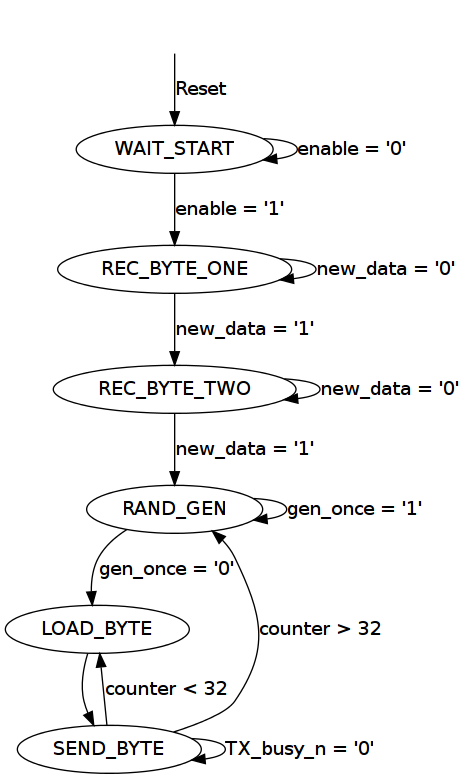
\includegraphics[scale=0.3]{graphviz/PRSG_state_diagram.png}
		\caption{Pseudo-random Number Generator State Machine}
	\end{figure}   

The state machine is a simple one to comprehend. In the WAIT\_START state, the module is looking at its \textit{enable} signal which when set indicates the beginning of the module's operations. In the REC\_BYTE\_ONE and REC\_BYTE\_TWO states, the module is reading the 2-byte seed value coming in from the UART. Once the seed value has been received, the module then computes the first random number in the RAND\_GEN state. The module then proceeds to send the 32-byte random number over the UART in the next set of 32 LOAD\_BYTE and SEND\_BYTE states. The byte to be transmitted is loaded in the \textit{data\_out} register during the LOAD\_BYTE state. In the first occurrence of this state, \textit{gen\_once} is set to '1' which states that the first number has been generated. The loaded byte is then transmitted over UART in the SEND\_BYTE state whenever the UART is free to transmit as indicated by the \textit{TX\_busy\_n} signal. Once the 32 bytes have been transmitted, the module goes back to the RAND\_GEN state and stays there to continuously generate the next random numbers, one every clock cycle.

\subsection{Generation and Verification of Prime Number Candidates}
Once the random number generator is set up, the next stage is to generate a candidate value to test for primality. The candidate is generated by taking a seed, which in this case is either a pseudo-random number from the generator or a previous candidate that has passed the primality test. The equation to generate the candidate is as follows: 

\begin{displaymath}
candidate = (seed * 2) + 1
\end{displaymath}

Once the candidate is calculated, the candidate must be tested to see if it is a prime number. To do this, the Rabin-Miller Primality test is implemented. The Rabin-Miller Primality test is a probabilistic method of determining if a number is prime. The test relies on the contrapositive of Fermat's little theorem, which states that for a prime number \textit{n}:

\begin{displaymath}
a^{n-1} \equiv 1\ (\textrm{mod}\ n)
\end{displaymath}

In order to perform the Rabin-Miller test, a random number \textit{a} is chosen such that $a \le candidate$ and the value of $n = candidate$. Since the Rabin-Miller test relies on the exponentiation and modulation of large numbers, and the RSA encryption algorithm relies on the same operation, some research was done into how the RSA encryption algorithm performs these operations efficiently. From this research, it was discovered that RSA uses a special type of multiplier, known as a Montgomery multiplier, that performs the exponentiation and modulation in one module. For this project, a Montgomery multiplier from Opencore was selected to be used.

The generation and verification is performed in the module \textit{generate\_chain.vhd}. The module is composed of a state machine with four states. The states are: IDLE, GEN\_CAND, CHECK, and PRINT. The state machine diagram is as follows:

	\begin{figure}[h]
		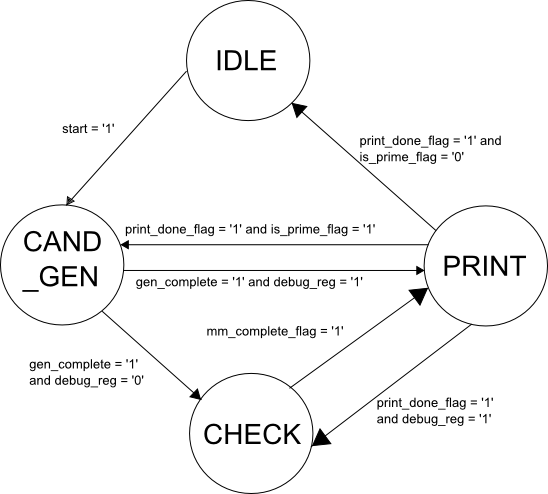
\includegraphics[scale=0.5]{diagrams/gen_chain_state.png}
		\caption{State diagram for generate\_chain.vhd}
	\end{figure}
	
The module starts in the IDLE state, waiting on the start bit input from the command parser to be set, indicating that the module should start generating a Cunningham chain. Once this bit is set, then the state machine transitions from the IDLE state to the GEN\_CAND state. This state is where the prime number candidate is generated. The candidate is generated by the value from the seed\_in\_reg, which is either the value from the random number generator or the previous candidate, shifting that value to the left by one bit, and appending a \textit{'1'} as the least significant bit. This operation is the same as multiplying the value in seed\_in\_reg by two and adding one to it.\\

Once the candidate is generated, the state machine either transitions to the PRINT state or the CHECK state, depending on whether or not the module is in debug mode. Debug mode is set through the input value debug, and its value stored in debug\_reg. If the module is not running in debug mode, then the state would transition to the CHECK state where the candidate is tested for primality. Otherwise, it will transistion to the PRINT state to print out values to help with programming and debugging. For the sake of brevity, the state transitions of the module in debug mode will be described. For the behavior of the module when not in debug mode, it is the same as the behavior in debug mode, sans this print state transition. Once the module is in the PRINT state, it will send out the character "S" followed by the value stored in seed\_in\_reg to the UART module, then it will send out the character "C" followed by the candidate value, again, to the UART module. A flag is then set that printing is complete.\\

When the printing is complete, the state machine then transitions to the CHECK state. The bahavior expressed in this paragraph is the expected behavior of the state, as the state was not implemented due to time constraints and issues that were encountered when interfacing with the Montgomery multiplier. In the check state, the module takes the value stored in seed\_in\_reg and sets that as the value of \textit{a}, and the candidate value as the value of \textit{n}. The Montgomery multiplier from Opencore takes in three values to perform the operation: \textit{a}, \textit{b}, and \textit{m}. These values are used as follows in the Montgomery multiplier: $a^b mod m$. The numbers that were chosen for \textit{a} and \textit{n} are then sent to the Montgomery multiplier, where $a = a$, $b = (n - 1)$, and $m = n$, and the Montgomery multiplier is started. The state then waits for the Montgomery multiplier to set a flag saying it is done computing. Once the Montgomery multiplier is done computing, then the result of the multiplier is checked. If the result is the value of 1, then the candidate is possibly a prime number. If the result is not the value of 1, then it is not a prime number. A flag is then set that checking of the candidate is complete.\\

Once the checking of the candidate is complete, the state machine transitions to the PRINT state. This time, the PRINT state will either send the value of the candidate to the UART module if it is a possible prime, or it will send the string "DONE" to the UART module if the candidate is not a possible prime. A flag is then set that printing is complete.\\

Once printing is complete, the state machine would then transition to either the IDLE state if the candidate was not a possible prime, or it would transition to the CAND\_GEN state if the candidate was a possible prime. Then the same behavior would then be repeated. Again, the state transitions described above are for when the module is in debug mode. The state transitions for the module in non-debug mode is the same, except for the first PRINT transition from CAND\_GEN.

\subsection{Verification of Generated Prime Numbers}
Since the prime number generators work on the principal of generating numbers that has a reasonably high probability of being prime, the numbers must be verified to insure that they are actually prime. This is a very resource intensive problem since it requires testing if the potential prime number number is evenly divisible by a set of numbers. Since it is prohibitively expensive to test if large prime numbers are definitively prime, probabilistic methods have been developed that will determine if a number is prime with a high probability. One of these probability methods of determining if a number is prime is called the Rabin-Miller primality test. \\

\subsubsection{Rabin-Miller Primality Test}
The Rabin-Miller primality test is a probabilistic method of determining if a number is prime. The algorithm is based around the idea of testing if a number in question is divisible by a subset of small primes. If it is not divisible by any of the small primes in the set then it is a prime number with a probability that is determined by the number of small primes in the set. The larger the set of small prime numbers is allows for the primality of the number in question to be determined with greater confidence. Since the probability of correctly identifying a prime number is directly related to the number of small primes tested again the test number, the accuracy of the Rabin-Miller primality test can be easily customized. \cite{cheung} \\

Now to dive into the theory of the Rabin-Miller primality test. The Rabin-Miller theory is based on the contrapositive of Fermat's little theorem which states that for a prime number \textit{n}:

	\begin{displaymath}
		a^{n-1} \equiv 1\ (\textrm{mod}\ n)
	\end{displaymath}

Therefore, the Rabin-Miller primality test can show that a number is not prime for a number \textit{n} if we can find a number \textit{a} such that:

	\begin{displaymath}
		a^d\ \textrm{mod}\ n\not \equiv 1\ or\ (n-1)
	\end{displaymath}
		
and

	\begin{displaymath}
		a^{2^rd}\ \textrm{mod}\ n \not \equiv (n-1)
	\end{displaymath}

for all $0 \le r \le s-1$, then \textit{n} is not prime if any such case is found. \cite{wiki_miller-rabin} \\

The Rabin-Miller Primality test is a good test to implement on hardware since the test can be parallelized by testing many small primes again the number in question concurrently and the math operations involved would be fairly expense in terms of cycles if implemented in software because of its sequential nature. Since we are attempting to implement this design in hardware let's first examine how to do the modulus operation in hardware. \\

One way to implement a modulus operation in hardware is to use the Montgomery algorithm to perform a modulo-multiply. These modulo-multiply operations can then be repeatedly run to perform an modular exponentiation. One potential issue with the modular exponentiation module is that it needs a pre-computed constant ($2^{2n}\ \textrm{mod}\ M$) to function. This isn't the worst thing since $M$ is the number we are testing if it is prime and $n$ is simply the number of bits in the multiplier. Therefore, this constant will be reused plenty when testing if a single number is prime. \\

As it turns out there are multiple ways to implement a Montgomery algorithm. The two major approaches are performing the multiplication first and then taking the modulus of the result or the other option is to do the multiplication and module operations in parallel. Since we are trying to implement this as efficiently as possible in hardware we will just focus on the designs that perform the multiplication and module operations in parallel. There are also many different ways to implement the multipliers used in the Montgomery algorithm. For brevities sake I will just discuss one of them here. For more information on some of the other possible configurations for the multipliers, please refer to reference: \cite{daly}. \\

Before I dive into the architecture for the Montgomery multiplier I am going to discuss, it is important to understand the theory behind its operation. A Montgomery multiplier works on the principal of using the fact that normal multiplication accumulates digit products in the intermediate steps of its operation and does modular reductions for this digit product as the multiplication operation is occurring. This is done by using the least significant bits of the intermediate result and performs an addition and shift operation on it to arrive at the next bit of the modular product result. 

Here is one possible algorithm that can be used to perform modular multiplication when the operation is $(A * B)\ mod\ M$. \\

\begin{lstlisting}
  Montgomery_Mod_Mult(A,B,M)
  {
    S[0] = 0;
    A = 2*A;
	  
    for{i=1; i <= n+1; i++}{
      q[i] = S[i-1] mod 2; //LSB of S[i-1]
      S[i] = (S[i-1] + q[i]*M + b[i]*A)/2;
    }
    return S;
  }
\end{lstlisting}

Now that we have some understanding for the algorithm behind a Montgomery multiplication we can move on to discussing a possible hardware implementation. One way to break this problem down is to focus on the two addition and two multiplication operations that are performed every round. We can break the problem down into an addition of $2A*b[i] + S[i-1]$ and $q[i]*M$ added to the sum of the previous operation. We can simplify the divide by two operation to simply eliminating the LSB from the next addition operation. Figure 1 portrays a block diagram for this particular implementation of the Montgomery multiplier. \\

	\begin{figure}[h]
		\centering
		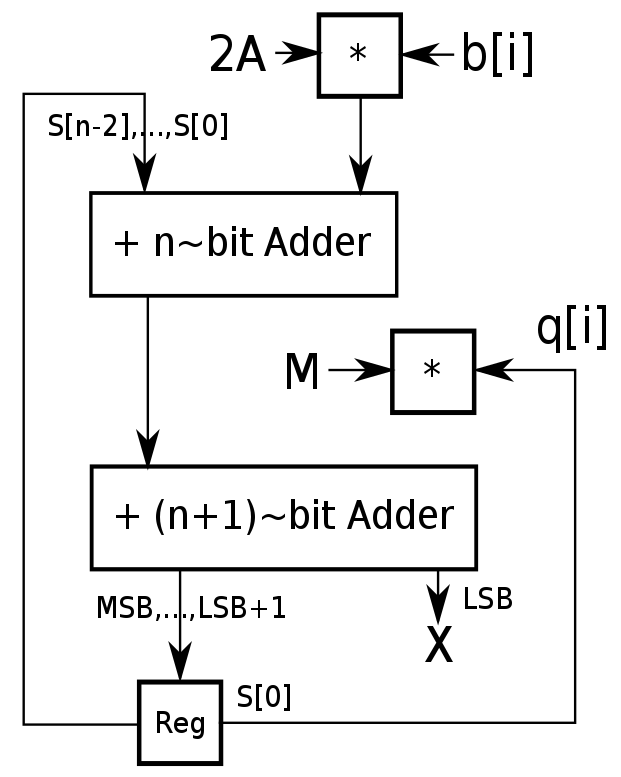
\includegraphics[scale=0.2]{pics/Montgomery_exp_mult.png}
		\caption{Montgomery Multiplier Block Diagram}
	\end{figure}   


Once the Montgomery multiplier is built, it is fairly easy to use the use the design to do exponential modulus operations as well. This is done by feeding the end result from the Montgomery multiplier back in as an input and repeating this pattern as many times as needed to arrive at the correct answer for the desired power. This is most clearly shown with an example.  

\begin{displaymath}
	32^3\ mod\ 7 = 32*((32*32)\ mod\ 7)\ mod\ 7
\end{displaymath}

To perform the given operation with the Montgomery multiplier, the first round of inputs would be:

\begin{displaymath}
	A = 32,\ \ B = 32,\ \ M = 7
\end{displaymath}

For the second round:

\begin{displaymath}
	A = (previous\ result),\ \ B=32,\ \ M=7
\end{displaymath}

Therefore, to perform a exponential modulus operation requires $(exponential\ power) - 1$ operations to complete using a single Montgomery multiplier. \\

There is another advantage to the algorithm chosen for verifying prime numbers.
The $a^{2^rd} \not \equiv (n-1)$ operation for all $0 \le r \le s-1$ can be performed by simply starting up the operation for $a^{2^{s-1}d}$ and comparing the results continuously at the correct cycle counts to determine if the number is prime. This saves the design from the penalty that would be occurred if the operation would have to be restarted for every new value of $r$. 

% needed in second column of first page if using \IEEEpubid
%\IEEEpubidadjcol

%\subsubsection{Subsubsection Heading Here}



% An example of a floating figure using the graphicx package.
% Note that \label must occur AFTER (or within) \caption.
% For figures, \caption should occur after the \includegraphics.
% Note that IEEEtran v1.7 and later has special internal code that
% is designed to preserve the operation of \label within \caption
% even when the captionsoff option is in effect. However, because
% of issues like this, it may be the safest practice to put all your
% \label just after \caption rather than within \caption{}.
%
% Reminder: the "draftcls" or "draftclsnofoot", not "draft", class
% option should be used if it is desired that the figures are to be
% displayed while in draft mode.
%
%\begin{figure}[!t]
%\centering
%\includegraphics[width=2.5in]{myfigure}
% where an .eps filename suffix will be assumed under latex, 
% and a .pdf suffix will be assumed for pdflatex; or what has been declared
% via \DeclareGraphicsExtensions.
%\caption{Simulation Results.}
%\label{fig_sim}
%\end{figure}

% Note that IEEE typically puts floats only at the top, even when this
% results in a large percentage of a column being occupied by floats.


% An example of a double column floating figure using two subfigures.
% (The subfig.sty package must be loaded for this to work.)
% The subfigure \label commands are set within each subfloat command,
% and the \label for the overall figure must come after \caption.
% \hfil is used as a separator to get equal spacing.
% Watch out that the combined width of all the subfigures on a 
% line do not exceed the text width or a line break will occur.
%
%\begin{figure*}[!t]
%\centering
%\subfloat[Case I]{\includegraphics[width=2.5in]{box}%
%\label{fig_first_case}}
%\hfil
%\subfloat[Case II]{\includegraphics[width=2.5in]{box}%
%\label{fig_second_case}}
%\caption{Simulation results.}
%\label{fig_sim}
%\end{figure*}
%
% Note that often IEEE papers with subfigures do not employ subfigure
% captions (using the optional argument to \subfloat[]), but instead will
% reference/describe all of them (a), (b), etc., within the main caption.


% An example of a floating table. Note that, for IEEE style tables, the 
% \caption command should come BEFORE the table. Table text will default to
% \footnotesize as IEEE normally uses this smaller font for tables.
% The \label must come after \caption as always.
%
%\begin{table}[!t]
%% increase table row spacing, adjust to taste
%\renewcommand{\arraystretch}{1.3}
% if using array.sty, it might be a good idea to tweak the value of
% \extrarowheight as needed to properly center the text within the cells
%\caption{An Example of a Table}
%\label{table_example}
%\centering
%% Some packages, such as MDW tools, offer better commands for making tables
%% than the plain LaTeX2e tabular which is used here.
%\begin{tabular}{|c||c|}
%\hline
%One & Two\\
%\hline
%Three & Four\\
%\hline
%\end{tabular}
%\end{table}


% Note that IEEE does not put floats in the very first column - or typically
% anywhere on the first page for that matter. Also, in-text middle ("here")
% positioning is not used. Most IEEE journals use top floats exclusively.
% Note that, LaTeX2e, unlike IEEE journals, places footnotes above bottom
% floats. This can be corrected via the \fnbelowfloat command of the
% stfloats package.



\section{Conclusion}
Producing Cunningham chains is a very computationally intensive problem that can be greatly parallelized. This type of problem is perfectly suited for an FPGA. Also, there is great value in producing Cunningham chains. Cunningham chains are greatly valued for in the fields of prime number research and cryptocurrency. Also, very large validated prime numbers are critical in many areas of the security field. Hence, parts of this project can be used for multiple useful applications in various domains. Through this project we hope to make our own small but meaningful contribution to these areas.

% if have a single appendix:
%\appendix[Proof of the Zonklar Equations]
% or
%\appendix  % for no appendix heading
% do not use \section anymore after \appendix, only \section*
% is possibly needed

% use appendices with more than one appendix
% then use \section to start each appendix
% you must declare a \section before using any
% \subsection or using \label (\appendices by itself
% starts a section numbered zero.)
%


%\appendices
%\section{Proof of the First Zonklar Equation}
%Appendix one text goes here.

% you can choose not to have a title for an appendix
% if you want by leaving the argument blank
%\section{}
%Appendix two text goes here.


% use section* for acknowledgement
%\section*{Acknowledgment}


%The authors would like to thank...


% Can use something like this to put references on a page
% by themselves when using endfloat and the captionsoff option.
\ifCLASSOPTIONcaptionsoff
  \newpage
\fi




% trigger a \newpage just before the given reference
% number - used to balance the columns on the last page
% adjust value as needed - may need to be readjusted if
% the document is modified later
%\IEEEtriggeratref{8}
% The "triggered" command can be changed if desired:
%\IEEEtriggercmd{\enlargethispage{-5in}}

% references section

% can use a bibliography generated by BibTeX as a .bbl file
% BibTeX documentation can be easily obtained at:
% http://www.ctan.org/tex-archive/biblio/bibtex/contrib/doc/
% The IEEEtran BibTeX style support page is at:
% http://www.michaelshell.org/tex/ieeetran/bibtex/
%\bibliographystyle{IEEEtran}
% argument is your BibTeX string definitions and bibliography database(s)
%\bibliography{IEEEabrv,../bib/paper}
%
% <OR> manually copy in the resultant .bbl file
% set second argument of \begin to the number of references
% (used to reserve space for the reference number labels box)
\begin{thebibliography}{1}

\bibitem{cheung}
Cheung, R., Brown, A., Luk, W., Cheung, P.: A scalable hardware architecture for prime number validation. In: IEEE Int. Conf. on Field-Programmable Technology, pp. 177-184 (2004)

\bibitem{daly}
A. Daly and W. Mamane. Efficient architectures for implementing montgomery modular multiplication and RSA modular exponentiation on reconfigurable logic. In \textit{Tenth ACM International Symposium on Field-Programmable Gate Arrays} pages 40-49, February 2002.

\bibitem{wiki_miller-rabin}
Miller-Rabin Primality Test. On: \textit{Wikipedia}, 27 Oct. 2014. $<$http://en.wikipedia.org/wiki/Miller\%E2\%80\%93Rabin\_primality\_test$>$

\bibitem{primecoin}
S. King. (2007, July 7). Primecoin: Cryptocurrency with Prime Number Proof-of-Work(\textit{1st ed.})[Online] Available:http://primecoin.io/bin/primecoin-paper.pdf

\bibitem{polandPrime}
Szecowka, Przemysław M., and Wojciech Buszko, "Digital hardware for prime numbers generation" in \textit{Mixed Design of Integrated Circuits and Systems, 2012 Proceedings of the 19th International Conference}, Warsow, Poland, MIXDES 2012.

\bibitem{ausPrime}
Saleeba, Michael and Pose, Ronald, "A Fast Algorithm for Prime Number Generation using Dynamically Reconfigurable Logic", Clayton, Australia.


\end{thebibliography}

% biography section
% 
% If you have an EPS/PDF photo (graphicx package needed) extra braces are
% needed around the contents of the optional argument to biography to prevent
% the LaTeX parser from getting confused when it sees the complicated
% \includegraphics command within an optional argument. (You could create
% your own custom macro containing the \includegraphics command to make things
% simpler here.)
%\begin{IEEEbiography}[{\includegraphics[width=1in,height=1.25in,clip,keepaspectratio]{mshell}}]{Michael Shell}
% or if you just want to reserve a space for a photo:

%\begin{IEEEbiography}{Michael Shell}
%Biography text here.
%\end{IEEEbiography}

% if you will not have a photo at all:
%\begin{IEEEbiographynophoto}{John Doe}
%Biography text here.
%\end{IEEEbiographynophoto}

% insert where needed to balance the two columns on the last page with
% biographies
%\newpage

%\begin{IEEEbiographynophoto}{Jane Doe}
%Biography text here.
%\end{IEEEbiographynophoto}

% You can push biographies down or up by placing
% a \vfill before or after them. The appropriate
% use of \vfill depends on what kind of text is
% on the last page and whether or not the columns
% are being equalized.

%\vfill

% Can be used to pull up biographies so that the bottom of the last one
% is flush with the other column.
%\enlargethispage{-5in}



% that's all folks
\end{document}


